\documentclass[a4paper,11pt]{report}
\usepackage[T1]{fontenc}
\usepackage[utf8]{inputenc}
\usepackage[francais]{babel}
\usepackage[babel=true,kerning=true]{microtype}
\usepackage[usenames,dvipsnames,svgnames,table]{xcolor}
\usepackage[colorlinks,linkcolor={blue!30!black},citecolor={blue!50!black},urlcolor={blue!80!black}]{hyperref}
\usepackage{amsmath,amsfonts,amssymb,array,graphicx,caption,lmodern,subcaption,tikz,url,xspace,wrapfig}
\usepackage{textcomp,rotating,epic,pdfpages,listings,diagbox,multirow,float}
\usepackage{pgfplots}
\pgfplotsset{width=7cm,compat=1.8}

\usepackage[top=25mm,bottom=25mm,left=25mm,right=25mm]{geometry}

\parskip=6pt % adds vertical space between paragraphs

\begin{document}

\pagenumbering{gobble}  % Pas de numérotation
\begin{titlepage}
    \vspace*{50px}
    
\includegraphics[height=80px]{Images/logo_phelma.pdf}
    \vspace*{-80px}
\begin{flushright}
%     \vspace*{60px}
    
\includegraphics[height=65px]{Images/CIME.jpg}
\end{flushright}

\vspace*{2cm}

\begin{center}
\rule{\linewidth}{0.5mm}\\[0.4cm]
{\huge{\bfseries Compte Rendu}\\[0.4cm]
\textsc{TP Simulation électronique}\\[0.4cm]}
\rule{\linewidth}{0.5mm}\\[0.5cm]

\LARGE{\textsc{Nicolas Paillet, Félix Piédallu \& Giulia Rizzo}}\\[0.7cm]
\large{\textsc{2015-2016}}\\[2cm]

\Large{~}\\[1cm]
% 
\includegraphics[width=0.4\textwidth]{Images/CIME.jpg}\\[1cm]
%
 \large{Encadrant : Marco Pala}\\[2cm]
%

\end{center}
\end{titlepage}

\tableofcontents        % Table des matières avec liens, générée automatiquement.
\newpage
\pagenumbering{arabic}  % Numérotation de retour !


\chapter*{Introduction}
\addcontentsline{toc}{chapter}{Introduction}
La fabrication de composants microélectroniques devient, lorsqu'on diminue la dimension, de plus en plus critique en terme de qualité. En effet, on va être sensibles à différents effets qui vont s'accentuer à faible dimension:
\begin{itemize}
    \item Les courants de fuite par la grille, qui s'accentuent à faible dimension par effet tunnel (lorsque l'épaisseur d'oxyde passe en dessous de 1,2nm)
    \item Les effets de canaux courts qui apparaissent lorsque la largeur de la grille diminue.
    \item La rugosité des interfaces, notamment canal/grille, va voir son impact sur les performances augmenter
\end{itemize}

De plus, plus un composant est petit, plus la précision relative de fabrication va diminuer: les dimensions vont perdre en précisions, tandis que l'implantation et la diffusion de dopants dans le canal va apporter des processus aléatoires supplémentaires, à des échelles comparables aux dimensions des composants.

Pourtant, un processeur nécessite d'avoir des milliards de transistors de performances constantes, notamment une tension de seuil qui devra être la plus constante possible sur l'ensemble des transistors.

L'industrie microélectronique nécessite donc de caractériser parfaitement les transistors fabriqués. Le but de ce TP est donc de nous familiariser avec les techniques de caractérisation électronique, ainsi que de nous fournir un aperçu des performances des différentes technologies de transistors.

Nous avons à disposition des transistors BULK et FDSOI, de dimensions de grilles entre $30nm$ et $10\mu m$.

\chapter{Rappels des équations}

Avant tout, un petit rappel des équations caractérisant un transistor est nécessaire. On s'intéresse essentiellement au régime linéaire du transistor, donc en forte inversion.

\begin{itemize}
    \item Le courant de drain en fonction des tensions est donné par:
        \[I_d (V_g, V_d) = \frac{W}{L} \cdot \mu_{eff}(V_g) \cdot Q_i(V_g) \cdot V_d\] 
    \item avec l'inversion de charge en inversion forte:
        \[Q_i(V_g) \simeq C_{ox}(V_g - V_T - \frac{V_d}{2})\]
    \item et la mobilité effective en inversion forte:
        \[\mu_{eff}(V_g) =\frac{\mu_0}{1+\theta_1 (V_g - V_T - \frac{V_d}{2}) 
                                        +\theta_2 (V_g - V_T - \frac{V_d}{2})^2} \]

        Avec ici $\theta_{\{1,2\}}$ les coefficients d'atténuation de la mobilité linéaire et quadratique, qui sont dus essentiellement à la diffusion par la rugosité de la surface de la grille. 
\end{itemize}

Il nous faut aussi rappeler les paramètres essentiels du transistor que nous allons étudier: 
\begin{itemize}
    \item La tension seuil $V_{th}$
    \item La transconductance ohmique:
        \[g_m (V_g) = \dfrac{\partial I_d}{\partial V_g}\]
    \item Le gain en transconductance:
        \[\beta = G_m = \dfrac{W}{L} \cdot C_{ox} \cdot \mu_0\]
\end{itemize}

Enfin, la fonction Y permet d'extraire le gain en transconductance et la tension seuil de façon plus précise et "automatisable" que par la transconductance ohmique. Elle est en fait basée sur la transconductance elle-même :
\[ Y(V_g) = \frac{I_d(V_g)}{\sqrt{g_m(V_g)}}
\]

On peut alors exprimer $Y(V_g)$ sous la forme suivante :
\[Y(V_g) = \frac{\beta}{1+ \theta_1 (V_g - V_T - \frac{V_d}{2})} \frac{V_d (V_g - V_{Th} - \frac{V_d}{2})}{\sqrt{\dfrac{\partial}{\partial V_g}(V_d \cdot C_{ox} (V_g - V_{Th} - \frac{V_d}{2}))}}
\]


\chapter{Mesure de la tension de seuil}
La tension de seuil est la caractéristique principale de fonctionnement du transistor. Elle déterminera la consommation du dispositif, ainsi que sa performance en terme de fréquence de fonctionnement. Il est donc nécessaire de caractériser correctement cette tension.

Notamment, la tension de seuil doit être un paramètre constant dans une production industrielle et surtout très bien déterminé pour les applications pour lesquelles le transistor est fait.

\section{Méthode de la transconductance}
Cette méthode repose sur la caractéristique $I_d$ en fonction de $V_g$. En effet, ce tracé permet de déterminer assez facilement $V_T$, graphiquement. Cependant, une méthode uniquement visuelle n'est pas systématique et fortement dépendante de l'opérateur donc non applicable en l'état.

Une autre méthode sera beaucoup plus adaptée à une caractérisation fiable, automatisée et constante:
\begin{enumerate}
    \item Tracé de la caractéristique $I_d = f(V_g)$
    \item Tracé de la dérivée $\frac{d I_d}{d V_g} = f(V_g)$
    \item On détermine alors le maximum de la dérivée et on trace la tangente à $I_d(V_g)$ en ce point.
    \item Le gain du transistor $\beta = G_m$ est alors la pente de cette tangente
    \item Cette tangente croise l'axe des abscisses en $V_T$.
\end{enumerate}

Nous allons donc tracer les caractéristiques de transistors des deux technologies, en fixant $V_d = 50mV$.

\subsection{Transistor Bulk}
Nous n'avons pu tracer qu'une caractéristique de transistor Bulk, par manque de transistors fonctionnels (le jeu étant d'abord de trouver un transistor qui n'ait pas déjà été grillé par les groupes précédents).

La figure \ref{transconductance bulk} représente le tracé de la transconductance pour un transistor Bulk de longueur de grille $40\mu m$.

\begin{figure}[h]
    \begin{center}
        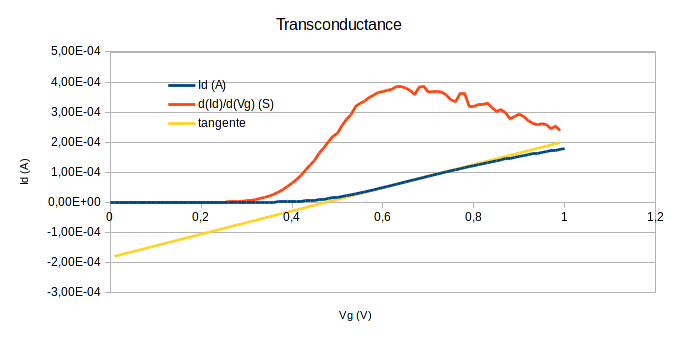
\includegraphics[width=0.8\textwidth]{Images/Bulk40-Transconductance}
        \caption{Transconductance du transistor Bulk, $l=40\mu m$, $V_d = 50mV$}
        \label{transconductance bulk}
    \end{center}
\end{figure}

Le maximum de la dérivée est atteint pour $V_g = 0,69V$, on peut alors déterminer:
\begin{itemize}
    \item Le gain du transistor $\beta = G_m = 386\mu S$
    \item $V_T(Bulk, 40\mu m) = 0,47V$
\end{itemize}


\subsection{Transistor FDSOI}
Nous pouvons réaliser la même étude sur des transistor FDSOI.

La figure \ref{transc_fdsoi_10um} permet de mesurer:

\begin{itemize}
    \item Le gain du transistor pour $V_g = 0,62V$: $\beta = G_m = 700\mu S$
    \item La tension seuil: \[V_T(FDSOI, 10\mu m) = 0,5V\]
\end{itemize}

\vspace*{8mm}
Et la figure \ref{transc_fdsoi_30nm} nous donne:
\begin{itemize}
    \item Le gain du transistor pour $V_g = 0,8V$: $\beta = G_m = 500\mu S$
    \item La tension seuil: \[V_T(FDSOI, 30nm) = 0,37V\]
\end{itemize}



\begin{figure}[h]
    \begin{center}
        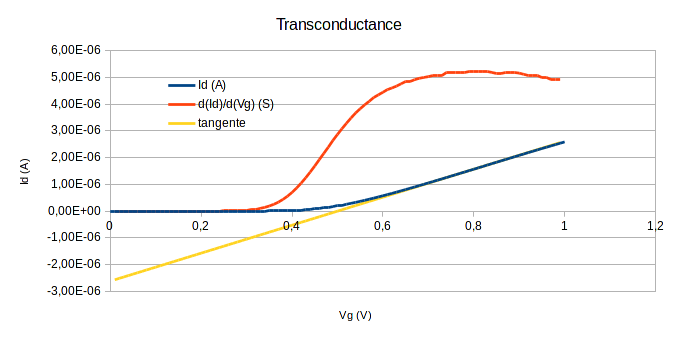
\includegraphics[width=0.8\textwidth]{Images/FD1-10-Transconductance}
        \caption{Transconductance du transistor FDSOI, $l=10\mu m$, $V_d = 50mV$}
        \label{transc_fdsoi_10um}
    \end{center}
\end{figure}
\begin{figure}[h]
    \begin{center}
        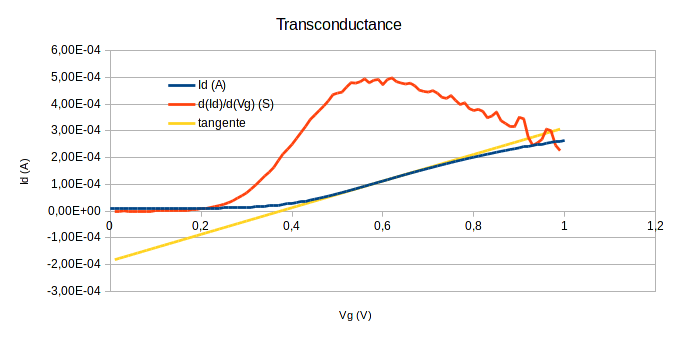
\includegraphics[width=0.8\textwidth]{Images/FD11-30-Transconductance}
        \caption{Transconductance du transistor FDSOI, $l=30nm$, $V_d = 50mV$}
        \label{transc_fdsoi_30nm}
    \end{center}
\end{figure}



\section{Méthode de la fonction Y}
On peut également utiliser une méthode différente pour déterminer $V_T$, à l'aide d'une fonction Y, définie par:
\[Y(V_g)=\dfrac{I_d(V_g)}{\sqrt{g_m(V_g)}}\]

Cette fonction est linéaire après le seuil, on peut alors approximer asymptotiquement plus précisément. On obtient alors $V_T$.
\subsection{Transistor Bulk}
\begin{figure}[h]
    \begin{center}
        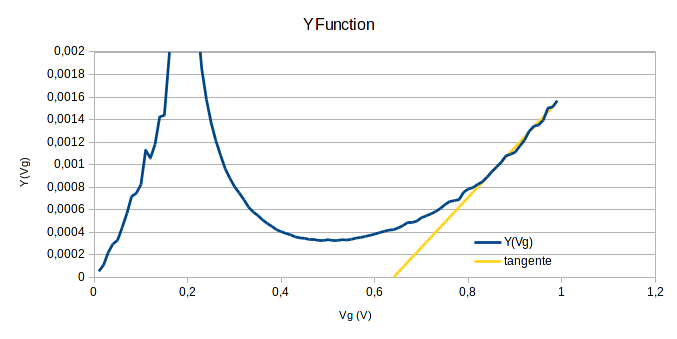
\includegraphics[width=0.8\textwidth]{Images/Bulk40-YFunction}
        \caption{Fonction Y du transistor Bulk, $l=40\mu m$, $V_d = 50mV$}
        \label{yfun_bulk_40}
    \end{center}
\end{figure}

On remarque ainsi dans la figure \ref{yfun_bulk_40} que la tension de seuil pour le transistor Bulk de $40\mu m$ vaut $650mV$, valeur légèrement supérieure à ce que nous avons déterminé précédemment.

\subsection{Transistor FDSOI}
\begin{figure}[h]
    \begin{center}
        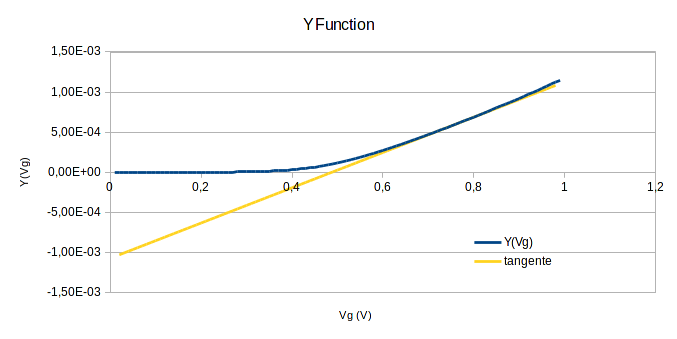
\includegraphics[width=0.8\textwidth]{Images/FD1-10-YFunction}
        \caption{Fonction Y du transistor FDSOI, $l=10\mu m$, $V_d = 50mV$}
        \label{yfun_fdsoi_10um}
    \end{center}
\end{figure}
\begin{figure}[h]
    \begin{center}
        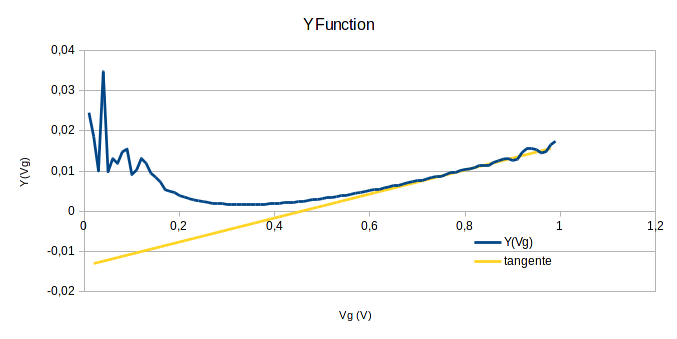
\includegraphics[width=0.8\textwidth]{Images/FD11-30-YFunction}
        \caption{Transconductance du transistor FDSOI, $l=30nm$, $V_d = 50mV$}
        \label{yfun_fdsoi_30nm}
    \end{center}
\end{figure}

Pour les transistors FDSOI, on obtient (Figure \ref{yfun_fdsoi_10um}) $V_T=490mV$ pour le transistor de 10 $\mu m$ et (Figure \ref{yfun_fdsoi_30nm}) $V_T=450mV$ pour celui de $30nm$. Ces valeurs sont sensiblement différentes des valeurs précédentes.


\section{Méthode du courant constant}
À $V_d$ fort, il n'est plus possible de trouver grâce à la méthode de la transconductance. On utilise alors une méthode dite du courant constant. Elle consiste à trouver un courant de seuil $I_{d_{TH}}$ pour $V_d$ faible, qui correspond au courant à $V_T$, puis de considérer la relation: \[I_{d_{TH}}=I_{d_{N}}\cdot\dfrac{W}{L}\]

$I_{d_{N}}$ est alors un paramètre arbitraire, un critère, que l'on pourra utiliser pour une série de transistors dont les dimensions seront différentes, afin de déterminer $V_T$ de manière uniforme.


\subsection{Transistor FDSOI}
%TODO graphe

%TODO calculs

\chapter{Mesure du DIBL}
Le DIBL est également important à connaître car il peut sensiblement modifier les performances du transistor. C'est un effet qui apparait lorsque les  longueurs de grille du transistor deviennent faibles. En effet, il arrive un moment dans la réduction de la longueur de grille où la tension appliquée $V_D$ a un influence sur la tension de seuil. 
On peut le calculer à partir des données précedentes.
\[ DIBL = -\frac{V^{DD}_{Th} - V^{low}_{Th}}{V_{DD} - V^{low}_{D}}
\]

\begin{figure}[h]
    \begin{center}
        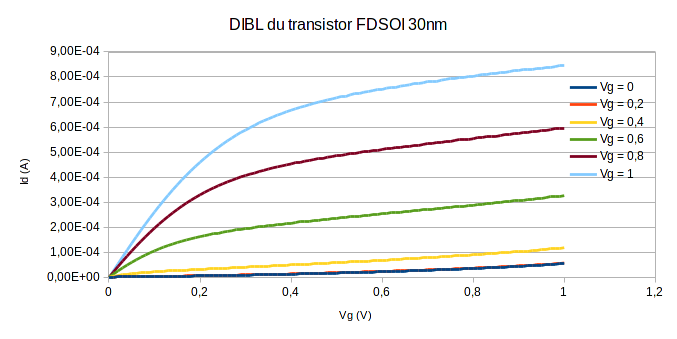
\includegraphics[width=0.8\textwidth]{Images/DIBL-11-30}
        \caption{$I_d(V_g)$ du FDSOI, $l = 30nm$}
        \label{DIBL_fdsoi_30nm}
    \end{center}
\end{figure}


\begin{figure}[h]
    \begin{center}
        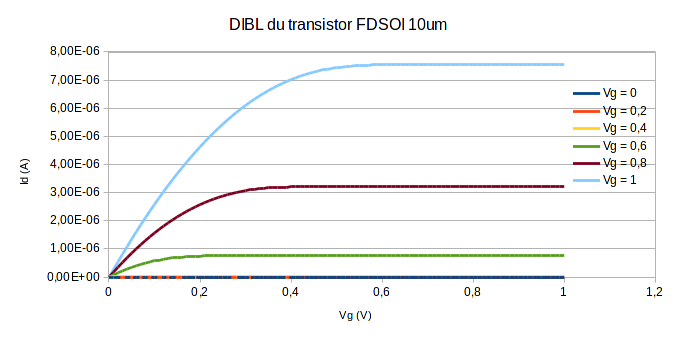
\includegraphics[width=0.8\textwidth]{Images/DIBL-1-10}
        \caption{$I_d(V_g)$ du FDSOI, $l =10\mu m$}
        \label{DIBL_fdsoi_10um}
    \end{center}
\end{figure}
%TODO calculs
On peut vérifier ces calculs en regardant la cours en log.
%TODO graphe
On peut également voir l'effet du DIBL en traçant des caractéristiques $I_d(V_d)$.
%TODO graphe 

\section{Comparaison des architectures}

\chapter*{Conclusion}
\addcontentsline{toc}{chapter}{Conclusion}

Ce TP nous a permis de découvir plus en détails la caractérisation électronique que nous avions abordé l'an passé en caractérisant des diodes et des capacités. Nous avons ainsi pu observer le comportement electrique de différents transistors (Architecture bulk et FDSOI) de taille différentes et d'étudier leurs performances. De plus ce TP est un complément aux cours de composants car il permet de visualiser en pratique les résultats affirmés en cours. Nous avons pu mesurer les caractéristiques tracées à main levée en cours et trouver les caractéristiques des transistors, mesures classiques en microéléctroniques.

















\end{document}
